This section describes the speedup of the GPU version of DENDRO with respect to the CPU version. Speedup is compared according to the steps which are described in the methodology section using the NVIDIA GTX 1060 GPU with 6GB of memory capacity. Average computational time is taken for the execution of five blocks in different levels within a confidence interval of 95\%.

\begin{figure}
  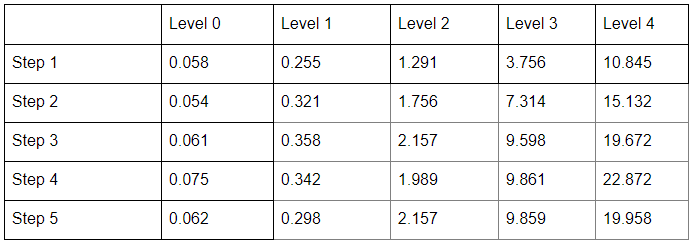
\includegraphics[width=\linewidth]{./images/table.png}
  \caption{Speedup of different steps}
  \label{fig:table}
\end{figure}


% \subsection{Step 1}
% First implementation of the CUDA code for DENDRO does not consider the GPU specific optimizations. According to the results in the Figure \ref{fig:table}, it can be observed that when the size of the data block is smaller (specially for level 0, level 1 and level 2 blocks), there is no any speedup. Even though the processing of data points in blocks is done in parallelly, overhead of data transfer time has beaten the gain from parallel execution. But for the processing of data blocks of level 3 and beyond, significant speedup can be seen in this approach as well as in the other four approaches. GPU should have enough work with respect to the memory transfer overhead to gain a remarkable speedup. Therefore, larger the block size larger the speedup that can be gained.

% \subsection{Step 2}
% For the second step, optimization of the cache of the GPU is considered. In this approach, data required for the processing of one block is bundled together in order to increase the cache hit rate. Figure \ref{fig:table} shows the running time and the speedup results for that execution. With this implementation, the speedup increased compared to step 1.

% \subsection{Step 3}
% In the third step, one-time memory allocation is introduced for the intermediate arrays as a further improvement to the step 2. For the previous steps, memory allocation tasks are carried out for the execution of one block and they are also deallocated subsequently. After these memory allocations and deallocations are removed, the speedup that is shown in the Figure \ref{fig:table} could be able to achieve. Memory allocation and deallocation functions are blocking functions. Therefore, remarkable speedup is achieved for all the data block sizes especially when the larger data blocks are processed.

% \subsection{Step 4}
% In this step, asynchronous data transfer technique was introduced to step 3. By doing that, a significant speedup was gained especially for larger data block sizes as shown in Figure \ref{fig:table}. While processing is going on for one block, data required to process the next block is sent to the GPU. Output data is also taken back to the host memory in similar passion. This approach allows to eliminate all the back and forth data transfer cost except for the first and last data block.

% \subsection{Step 5}
% As the fifth step, implementation of fourth step was improved by making memory copying of host to device and device to host in parallel. In order to do that pinned memory is required to get the output of GPU. Allocating pinned memory has its own computational overhead. But considering the profiling timeline of step 4 and step 5 (Figure \ref{fig:kernal_memcpy_overlap} and Figure \ref{fig:duel_mem_cpy}), It can be seen that the computational process is dominating over the memory transfer time in both steps. Which means that the bottleneck is not the memory copying process. Hence improving memory copying performance will not affect to the overall performance while performance of computational process stays the same.  But due to the overhead of pinned memory allocation, this approach failed to achieve the performance of approach of step 4.